\chapter{Goals}
\label{chapter:Goals}
One of our goals is to develop a graphical editor for music generation. With its help it will be possible to create patches, test their output in a simulation and produce a netlist to generate that sound on an \ac{FPGA}. A patch consists of different sound-components like wave generators and filters. In order to create specific sounds, the sound-components have to be connected. The exported netlist can be put on an \ac{FPGA} so the user of the synthesizer (e.g. a musician) can connect a MIDI device or specific sensors to the \ac{FPGA} to modify input values at runtime. %first appearance of FPGA, therefore "a FPGA"

To describe the functions which we want to develop in detail, the following section will provide use case diagrams and their description.

\section{Editor for the designer}
\label{editor}
Figure \ref{fig:Soundgate_Designer} shows the use cases for the editor.

	\begin{figure}[!h]
		\centering
			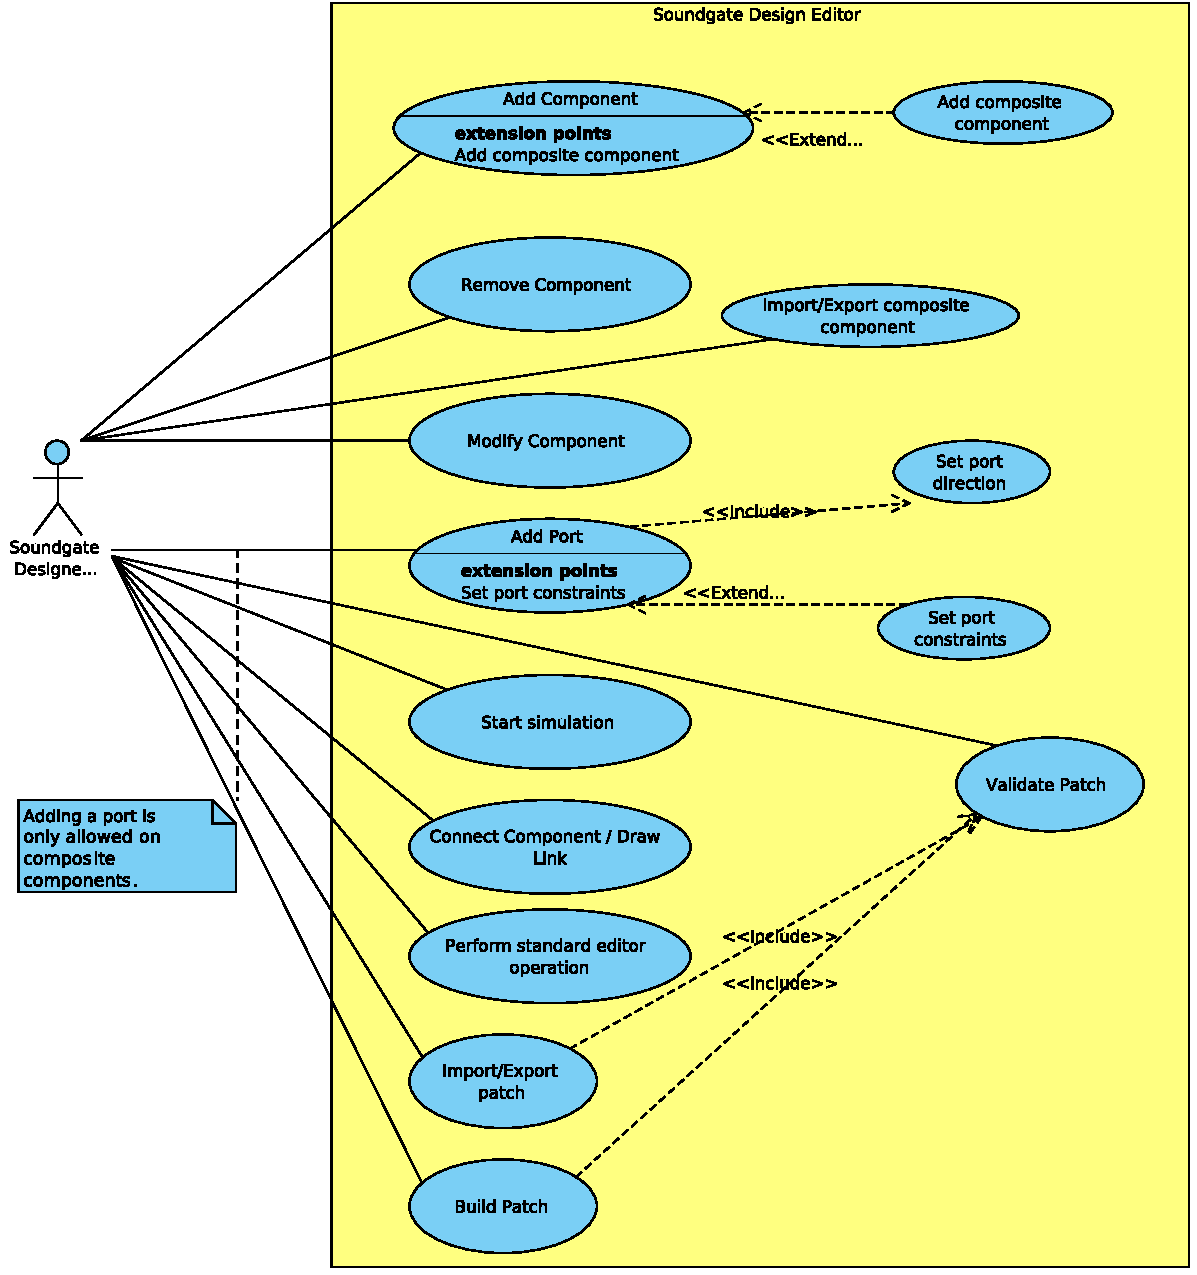
\includegraphics[width=1\textwidth]{images/Soundgate_Designer.pdf}
		\caption{Use case diagram for the Soundgate editor}
		\label{fig:Soundgate_Designer}
	\end{figure}

In the editor the designer can create new patches, open existing ones and save them.
He can add and remove sound-components from the patch and connect the sound-components by drawing links between their ports.
A sound-component can either be an atomic or a composite component. 
Atomic sound-components are stored within XML-libraries and represent waveform generators, filters, etc; their ports are predefined. 
The ports of an atomic sound-component are mapped to its dynamic properties. Therefore a dynamic property changes according to the signal the mapped port receives.  
Some of these sound-components may have static properties which the designer can modify (e.g. the value of a constant-block) at design time, but cannot be changed during runtime. 

In contrast to atomic sound-components, composite sound-components are not predefined. 
The designer can add composite sound-components to the patch and fill them with either atomic sound-components or other composite sound-components. The internal linkage of a composite sound-components is setup also by drawing links between the components.
The designer can add ports to a composite sound-components and define their direction and constraints. 
We want to make it possible to export finished composite sound-components as XML-files and to import existing ones to the editor such that different designers can exchange their sound-components.


Furthermore, the designer must define the interfaces of his patch. 
The interfaces are the points where the end-user interacts with the system. 
These can be MIDI-inputs, sensor values etc.

We also plan to implement an extra feature, which allows to estimate the area consumption of the patch on the hardware, such that the designer can check the size of his patch at any point of time. 
Once a patch is finished it can be validated. The program tests if all constraints are fulfilled (e.g. if all ports are connected and so on). Finally, the designer can generate VHDL-code from the XML-file.

Of course, all standard editor operations like selecting, moving objects etc. are supported.

\section{Simulator}

We want to develop a software simulator for patches such that the designer and the user can test the sound of the patch before loading it on an \ac{FPGA}. Figure \ref{fig:Soundgate_Simulator} shows the use cases for the Soundgate simulator.

	\begin{figure}[!h]
		\centering
			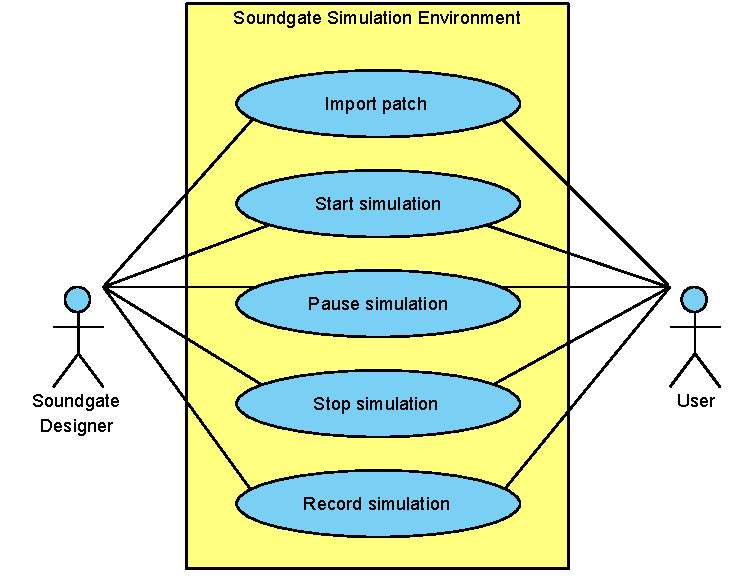
\includegraphics[width=0.90\textwidth]{images/Soundgate_Simulator.pdf}
		\caption{Use case diagram for the Soundgate simulation environment}
		\label{fig:Soundgate_Simulator}
	\end{figure}

A designer must be able to import a patch to the simulator and to start the simulation. Afterwards he is able to pause or stop the simulation. An optional feature we would like to implement is the possibility to save the output of a simulation to the HDD.

\section{COSMIC system}
	Figure \ref{fig:Soundgate_UserInterface} shows use cases for our so called \ac{COSMIC} system. 
	
	\begin{figure}[!h]
		\centering
			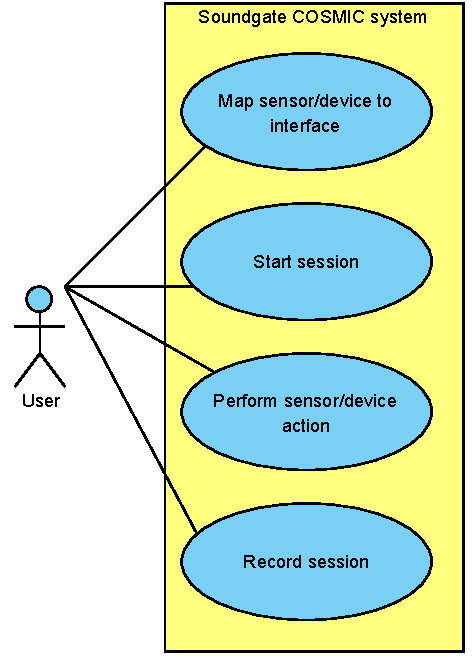
\includegraphics[width=0.50\textwidth]{images/User_View.pdf}
		\caption{Use case diagram of the Soundgate COSMIC system}
		\label{fig:Soundgate_UserInterface}
	\end{figure}
	
	As mentioned before, a patch created in the editor can be exported as an XML-file which is used to generate VHDL-code. 
	This VHDL-code is synthesized and put on an \ac{FPGA}. 
	The term \ac{COSMIC} refers to this final system, running on the \ac{FPGA}.
	
	The end-user (e.g. a musician or a performer) can then map sensor values and other inputs to the interfaces defined by the designer (see Section \ref{editor}). 
	The user starts the session by pushing a button. 
	During the session he performs some sensor actions or actions with other devices to create input values for the system.
	
\subsection{Input}
We will provide different ways of modifying the patch at runtime through sensors input. 
The first approach uses a device as a sensors whereas the other one will use the body of the musician, which will be tracked by a 3D depth camera. 
Apart from the control through sensors, the end-user should also be able to use MIDI devices, e.g. a keyboard.

\subsubsection{Mobile Device}
Today's mobile phones are full of different sensors which can easily be accessed with a small application. The Android SDK offers three different groups of sensors, namely:
\begin{itemize}
	\item \textbf{Motion Sensors} \\
			This group contains accelerometers, gravity sensors, gyroscope, and rotational vector sensors. % \todo{see ref to Android page}.
	\item \textbf{Environmental Sensors} \\
			With their help it is possible to check the air temperature, illumination and humidity.
	\item \textbf{Position Sensors} \\
			Orientation sensors and magnetometers.
\end{itemize}

Users can hardly control environmental sensors in a reliable way but depending on the scenario their values can still set the general mood of the sound.
The other sensors are perfectly suited for changing values interactively since they are modified simply by moving the phone and changing its orientation. 
We will develop an Android Application because the Android OS is widespread. 
On the one hand the sensors have to be read by the application and on the other hand these values have to be forwarded to the simulation environment. 
This can be done with Sockets to send these values over a network connection.

\subsubsection{3D depth camera}
A 3D camera like the Microsoft Kinect system is able to calculate the depth of an image. 
Therefore it is possible to track the movement of a person by tracking different joints, which have to be calibrated at the beginning. 
So it is possible to connect parameters of a sound-component i.e. the altitude, to one of the person's arms. 
This method abstracts the sensors so it feels like if the person himself is possible to change the sound.

\section{Open Sound Control}
The communication between the sensors and the entire system will be realized with ethernet and WiFi. 
Therefore it is possible to send different values to the \ac{FPGA} so it changes its parameters. 
Through \ac{ReconOS} and a Linux kernel it is possible to open a server socket to listen for those messages. 
However it is necessary to agree on a specific protocol. Instead of developing a protocol of our own, we are going to use the Open Sound Control Protocol.

The \ac{OSC} is a message based communication protocol. 
Signals can be created by different sensors and be sent to the receiver. 
Additionally it is transport protocol independent, so we could either use error detecting TCP or the faster UDP protocol. 
Since a device is capable of generating relatively big amounts of data per second, we are most likely forced to use UDP. 
If there is any packet loss or transmission error the users won't probably hear it since the sensors are continuously generating new values. 
Additionally we could use as many devices as the system could handle since it does not care about who is sending a message.

An \ac{OSC} message contains the target component of the synthesizer together with some new parameters. 
An example message, which would modify the frequency of a specific sine wave generator would look like this: 

\emph{/synthesizer1/oscillator/sine1/freq “int32” 440} \\


\section{Component library}
In order to create a patch in the first place, we provide the basic components that are necessary to build an advanced synthesizer. 
These components can also be combined to create new components.



	 \begin{tabular}[h]{|c|p{9.75cm}|}
	  \hline
	  Component & Description \\
	  \hline
	  \hline
	  Wave Generators & Basic soundwaves that create simple tones (e.g. sine, sawtooth, rectangular) \\\hline
		Basic Arithmetic functions & Components that support simple arithmetic operations on soundsignals (e.g. addition, multiplication)\\\hline
		Filters & Arithmetic functions can be combined to complex filters (e.g. low pass). Filters emphasize or eliminate some frequencies from a signal \\\hline
		Mixer & Used to mix several sound signals to one sound output \\\hline
		Constants & Defined inputs for components \\\hline
		Interactive Inputs & Inputs, that can be changed at runtime with interactive sensors \\\hline
		MIDI components & Stores a MIDI file and outputs the different frequencies \\\hline
		Sound output & All signals end up here in order to be sent to the \ac{DAC} and played on the speaker \\\hline
	 \end{tabular}
\\\\


Figure \ref{fig:ex_patch} depicts an example patch, which could be produced by the system. 
There are three different types of waveform generators (sine, sawtooth and rectangular), which are mixed in the Mixer. 
Each of the waveform generators has different possible inputs: 
First, the input of the sine waveform generator is predefined with 440\,Hz. 
The sawtooth waveform generator gets its input from an interactive sensor, which can be connected to the \ac{FPGA}. 
At last, there is a MIDI controller used for the rectangular waveform generator, which stores a MIDI file and outputs the frequencies of the file.
After mixing the waveforms, the signal is filtered by a low pass filter before it is played on the speaker. In this example, the low pass filter filters each frequency above the threshold of 600 Hz.

%\begin{itemize}
%\item Generators:
%\begin{itemize}
%\item sine
%\item Sawtooth
%\end{itemize}
%
%\item Filters:
%\begin{itemize}
%\item Ramp
%\item Low pass
%\item Delay
%\end{itemize}
%
%\item Arithmetic:
%\begin{itemize}
%\item Addition 
%\item Multiplication
%\item Equals
%\end{itemize}
%
%\item Mixer
%
%\item Sources:
%\begin{itemize}
%\item Constant
%\end{itemize}
%
%\item Sinks:
%\begin{itemize}
%\item Sound output
%\end{itemize}
%
%\item MIDI: 
%\begin{itemize}
%\item MIDI note to frequency converter
%\item MIDI scheduler
%\end{itemize}
%\end{itemize}
	\begin{figure}[!h]
		\centering
			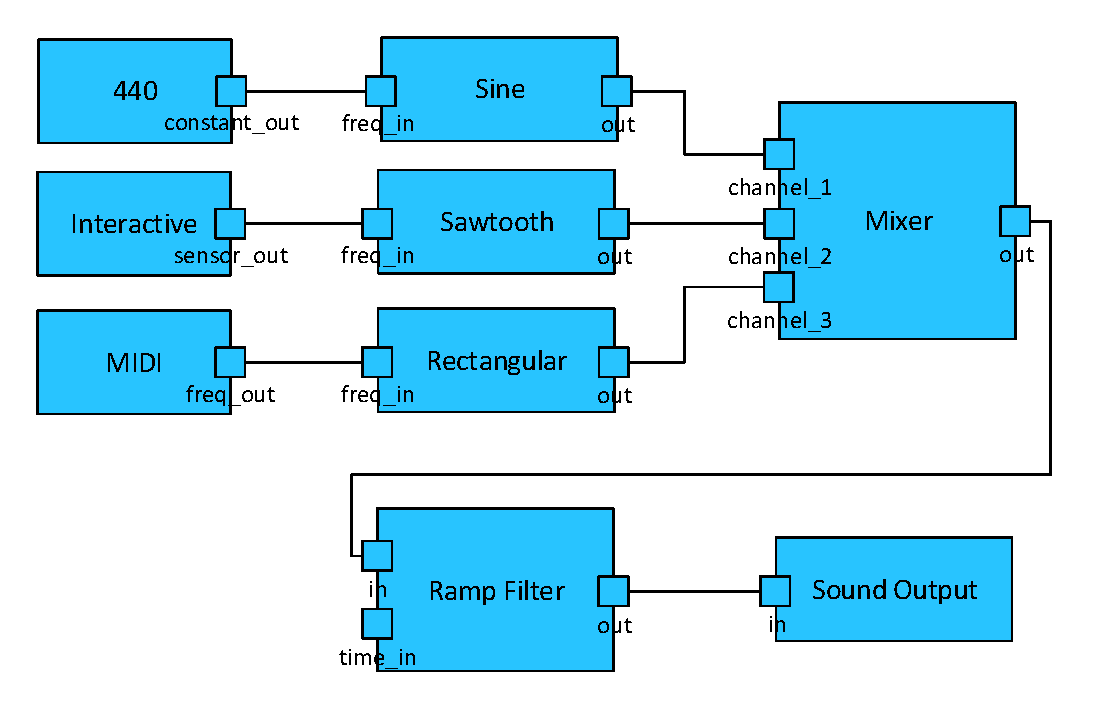
\includegraphics[width=\textwidth]{images/ex_patch.pdf}
		\caption{Example patch}
		\label{fig:ex_patch}
	\end{figure}

